\documentclass[journal]{IEEEtran}

% *** GRAPHICS RELATED PACKAGES ***
%
\ifCLASSINFOpdf
  \usepackage[pdftex]{graphicx}
   \usepackage{epstopdf}
  % declare the path(s) where your graphic files are
   \graphicspath{{../Imagens/}}
  % and their extensions so you won't have to specify these with
  % every instance of \includegraphics
  % \DeclareGraphicsExtensions{.eps}
\else
  % or other class option (dvipsone, dvipdf, if not using dvips). graphicx
  % will default to the driver specified in the system graphics.cfg if no
  % driver is specified.
  % \usepackage[dvips]{graphicx}
  % declare the path(s) where your graphic files are
  % \graphicspath{{../eps/}}
  % and their extensions so you won't have to specify these with
  % every instance of \includegraphics
  % \DeclareGraphicsExtensions{.eps}
\fi
   
% \graphicspath{{../Imagens/}}  

% *** INPUT PACKAGES ***
%
\usepackage[utf8]{inputenc} 
% permite introduzir os caracteres especiais, escrevendo normalmente (sem uso da contra-barra)

\usepackage[T1]{fontenc}
% codificação da fonte

% *** MATH PACKAGES ***
%
%\usepackage[cmex10]{amsmath}
\usepackage{amsmath}

\usepackage{amssymb}

% *** SUBFIGURE PACKAGES ***
\usepackage[tight,footnotesize]{subfigure}

\usepackage{color}

\usepackage[figurename=Fig.]{caption}
\usepackage[font=footnotesize]{subfig}

\usepackage{cite}

% *** LANGUAGE PACKAGES ***
%
\usepackage[brazilian]{babel}

% *** OTHERS PACKAGES ***
%
\usepackage{placeins}
\usepackage[inline]{enumitem}
\usepackage{comment}

% \renewcommand{\keywords}[1]{\textbf{\small{\textit{Palavras-chave~---}} #1}}
\newcommand{\keywords}[1]{\textbf{\small{\textit{Palavras-chave~---}} #1}}
\renewcommand{\abstract}[1]{\textbf{\small{\textit{Resumo~---}} #1}}

\input{/home/valdir/Dropbox/LaTeX/ComandosPersonalizados.tex}

\begin{document}

\title{Filtro Butterworth Implementado na\\ Topologia Sallen Key}

\author
{
  \IEEEauthorblockN
  {
    Valdir Pedrinho de Tomin Junior\\
    \IEEEauthorblockA
    {
      Anotações Pessoais\\
    }      
  }
}
\maketitle

% \abstract{}

% \keywords{}

\begin{figure}
 \centering
 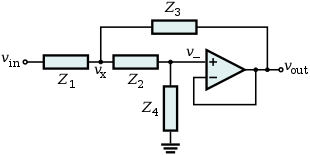
\includegraphics[width=0.45\textwidth]{Sallen-Key_Generic_Circuit} 
 \begin{eqnarray*} 
  Z_1 = R_1\quad
  Z_2 = R_2\quad
  Z_3 = \dfrac{1}{sC_1}\quad
  Z_4 = \dfrac{1}{sC_2}
 \end{eqnarray*}
 \begin{eqnarray*} 
  V_x = v_a(s)\quad
  Vin = v_i(s)\quad
  Vout = v_o(s)
 \end{eqnarray*}
 \begin{eqnarray*}
 \begin{aligned}
  & i_1(s) \textrm{ passa por } Z_1\quad
  i_2(s) \textrm{ passa por } Z_2 \textrm{ e } Z_4\\
  & i_3(s) \textrm{ passa por } Z_3
 \end{aligned} 
 \end{eqnarray*} 
 \caption{Topologia Sallen Key}
\end{figure}

\begin{equation}\label{eq_soma_correntes}
 i_1(s) = i_2(s) + i_3(s)
\end{equation}

% \begin{eqnarray*}
%  \begin{aligned}
%   & v_{\pc{+}} = i_2(s)\dfrac{1}{sC_2}\\
%   & v_{\pc{+}} = v_{\pc{-}} = v_o\\
%  \end{aligned}
% \end{eqnarray*}
% 
% \begin{equation}\label{eq_corrente_i2}
%  i_2(s) = C_2 s v_o(s)
% \end{equation}

\begin{align}
 & v_{\pc{+}} = i_2(s)\dfrac{1}{sC_2}\eqEndl
 & v_{\pc{+}} = v_{\pc{-}} = v_o\eqEndl
%  \eqEndl
 & i_2(s) = C_2 s v_o(s)\label{eq_corrente_i2}
\end{align}

% \begin{eqnarray}\label{eq_tensao_va}
%  \begin{aligned}
%   & v_a(s) = \pc{R_2+\dfrac{1}{sC_2}}i_2(s)\\
%   & v_a(s) = R_2C_2sv_o(s)+v_o(s)
%  \end{aligned}
% \end{eqnarray}

% \begin{equation}\label{eq_corrente_i1}
%  i_1(s) = \dfrac{v_i(s)-v_a(s)}{R_1}
% \end{equation}

\begin{align}
 & v_a(s) = \pc{R_2+\dfrac{1}{sC_2}}i_2(s)\eqEndl
%  \eqEndl
 & v_a(s) = R_2C_2sv_o(s)+v_o(s)\label{eq_tensao_va}
\end{align}


% \begin{eqnarray}\label{eq_corrente_i1}
%  \begin{aligned}
%   & i_1(s) = \dfrac{v_i(s)-v_a(s)}{R_1}\\
%   & i_1(s) = \dfrac{v_i(s)-R_2 C_2 sv_o(s)-v_o(s)}{R_1}
%  \end{aligned}
% \end{eqnarray}

% \begin{equation}\label{eq_tensao_v+}
%  v_{\pc{+}} = i_2(s)\dfrac{1}{sC_2}
% \end{equation}
% 
% \begin{equation}\label{eq_tensao_vo}
%  v_{\pc{+}} = v_{\pc{-}} = v_o
% \end{equation}
%  
% \begin{equation}\label{eq_corrente_i2}
%  i_2(s) = C_2 s v_o(s)
% \end{equation}

\begin{align}
 & i_1(s) = \dfrac{v_i(s)-v_a(s)}{R_1}\eqEndl
%  \eqEndl
 & i_1(s) = \dfrac{v_i(s)-R_2 C_2 sv_o(s)-v_o(s)}{R_1}\label{eq_corrente_i1}
\end{align}

% \begin{eqnarray}\label{eq_corrente_i3}
%  \begin{aligned}
%   & i_{3}(s)\dfrac{1}{sC_1} = v_a(s)-v_o(s)\\
%   & i_{3}(s) = sC_1\pr{v_a(s)-v_o(s)}\\
%   & i_3(s) = R_2C_1C_2s^2v_o(s)
%  \end{aligned}
% \end{eqnarray}

% \begin{equation}\label{eq_corrente_i1_II}
%  i_1(s) = \dfrac{v_i(s)-R_2 C_2 sv_o(s)-v_o(s)}{R_1}
% \end{equation}

% \begin{equation}\label{eq_corrente_i3_II}
%  i_3(s) = R_2C_1C_2s^2v_o(s)
% \end{equation}

\begin{align}
 & i_{3}(s)\dfrac{1}{sC_1} = v_a(s)-v_o(s)\eqEndl
 & i_{3}(s) = sC_1\pr{v_a(s)-v_o(s)}\eqEndl
%  \eqEndl
 & i_3(s) = R_2C_1C_2s^2v_o(s)\label{eq_corrente_i3}
\end{align}

% \begin{eqnarray}\label{eq_transf_func_vo/vi}
%  \begin{aligned}
%   & v_i(s)-R_2C_2sv_o(s)-v_o(s) = R_1C_2sv_o(s)+...\\&\quad+R_1R_2C_1C_2s^2v_o(s)\\
%   & v_i(s) = v_o(s)+sv_o(s)\pc{R_1C_2+R_2C_2}+...\\&\quad+s^2v_o(s)\pc{R_1R_2C_1C_2}\\
%   & \dfrac{v_o(s)}{v_i(s)} = \dfrac{1}{R_1R_2C_1C_2s^2+C_2\pc{R_1R_2}s+1}\\
%   & \dfrac{v_o(s)}{v_i(s)} = \dfrac{\dfrac{1}{R_1R_2C_1C_2}}{s^2+\dfrac{R_1+R_2}{R_1R_2C_1}s+\dfrac{1}{R_1R_2C_1C_2}}\\
%  \end{aligned} 
% \end{eqnarray}

\begin{align}
 & v_i(s)-R_2C_2sv_o(s)-v_o(s) = R_1C_2sv_o(s)+\eqBreak+R_1R_2C_1C_2s^2v_o(s)\eqEndl
 & v_i(s) = v_o(s)+sv_o(s)\pc{R_1C_2+R_2C_2}+\eqBreak+s^2v_o(s)\pc{R_1R_2C_1C_2}\eqEndl
 & H(s) = \dfrac{v_o(s)}{v_i(s)} = \dfrac{1}{R_1R_2C_1C_2s^2+C_2\pc{R_1R_2}s+1}\eqEndl
%  \eqEndl
 & H(s) = \dfrac{\dfrac{1}{R_1R_2C_1C_2}}{s^2+\dfrac{R_1+R_2}{R_1R_2C_1}s+\dfrac{1}{R_1R_2C_1C_2}}\label{eq_transf_func_vo/vi}
\end{align}

% \begin{equation}\label{eq_velocidade_angular_ao_quadrado}
%  \omega_{n}^2 = \dfrac{1}{R_1R_2C_1C_2}
% \end{equation}
% 
% \begin{equation}\label{eq_velocidade_angular}
%  \omega_{n} = \dfrac{1}{\sqrt{R_1R_2C_1C_2}}
% \end{equation}
% 
% \begin{equation}
%  \omega_{n} = 2\pi f_0
% \end{equation}

\begin{equation}\label{eq_transf_func_generica}
 H(s) = \dfrac{{\omega_0}^2}{s^2+2\zeta\omega_0 s+{\omega_0}^2}
\end{equation}

\begin{align}
 & \dfrac{\sqrt{2}}{2} = \md{\dfrac{{\omega_0}^2}{(j\omega_c)^2+2\zeta\omega_0 (j\omega_c)+{\omega_0}^2}}\eqEndl
 & \dfrac{\sqrt{2}}{2} = \md{\dfrac{{\omega_0}^2}{\pc{-{\omega_c}^2+{\omega_0}^2}+j\pc{2\zeta\omega_0\omega_c}}}\eqEndl
 & \dfrac{\sqrt{2}}{2} = \dfrac{\sqrt{\pc{{\omega_0}^2}^2}}{\sqrt{\pc{{\omega_0}^2-{\omega_c}^2}^2+\pc{2\zeta\omega_0\omega_c}^2}}\eqEndl
 & \dfrac{1}{2} = \dfrac{{\omega_0}^4}{\pc{{\omega_0}^2-{\omega_c}^2}^2+\pc{2\zeta\omega_0\omega_c}^2}\eqEndl
 & 2{\omega_0}^4 = \pc{{\omega_0}^2-{\omega_c}^2}^2+\pc{2\zeta\omega_0\omega_c}^2 \label{eq_veloc_angular_corte_generica}
\end{align}

% Onde $j = \sqrt{-1}$ e $\omega_c$ é a velocidadade angular de corte.


\begin{equation}\label{eq_fator_qualidade}
 Q = \dfrac{1}{2\zeta}
\end{equation}

\begin{align}
 & Q = \dfrac{\sqrt{2}}{2}\eqEndl
 & 2\zeta = Q^{-1} = \pc{\dfrac{\sqrt{2}}{2}}^{-1}\eqEndl
 & 2\zeta = \sqrt{2}\label{eq_2zeta_Butterworth}
\end{align}

\begin{align}
 & 2{\omega_0}^4 = \pc{{\omega_0}^2-{\omega_c}^2}^2+\pc{\sqrt{2}\omega_0\omega_c}^2\eqEndl
 & 2{\omega_0}^4 = {\omega_0}^4-2{\omega_0}^2{\omega_c}^2+{\omega_c}^4+2{\omega_0}^2{\omega_c}^2\eqEndl
 & {\omega_0}^4 = {\omega_c}^4\eqEndl
 & \omega_c = \omega_0\label{eq_veloc_angular_corte}
\end{align}



% \begin{equation}\label{eq_Q_Butterworth}
%  Q = \dfrac{\sqrt{2}}{2}
% \end{equation}




\begin{align}
 & \omega_{0}^2 = \omega_{c}^2 = \dfrac{1}{R_1R_2C_1C_2}\eqEndl
%  \eqEndl
 & \omega_{0} = \omega_{c} = \dfrac{1}{\sqrt{R_1R_2C_1C_2}}\label{eq_veloc_angular_natural}
\end{align} 
 
\begin{align} 
 & \omega_{0} = 2\pi f_0 = \omega_{c} = 2\pi f_c \eqEndl
 & 2\pi f_0 = 2\pi f_c = \dfrac{1}{\sqrt{R_1R_2C_1C_2}}\eqEndl
%  \eqEndl
 & f_0 = f_c = \dfrac{1}{2\pi \sqrt{R_1R_2C_1C_2}}\label{eq_freq_natural}
\end{align}

\begin{align}
 & 2\zeta\omega_0 = 2\zeta\pc{2\pi f_c} = \dfrac{R_1+R_2}{R_1R_2C_1} \eqEndl
 & 2\zeta = \dfrac{1}{2\pi f_c}\cdot\dfrac{R_1+R_2}{R_1R_2C_1}\cdot\dfrac{C_2}{C_2} \eqEndl
 & \dfrac{1}{2\zeta} = Q = \dfrac{2\pi f_cR_1R_2C_1C_2}{C_2\pc{R_1+R_2}} \eqEndl
 & Q = \dfrac{2\pi R_1R_2C_1C_2}{C_2\pc{R_1+R_2}} \cdot \dfrac{1}{2\pi\sqrt{R_1R_2C_1C_2}} \cdot \dfrac{2\pi}{2\pi} \eqEndl
 & Q = \dfrac{{f_c}^{-2} f_c}{2\pi C_2\pc{R_1+R_2}} \eqEndl
 & Q = \dfrac{1}{2\pi f_c C_2\pc{R_1+R_2}} \label{eq_Q_Butterworth}
\end{align}


Equações do software:\\

\begin{equation}\label{eq_alpha}
 \alpha = R_1R_2C_1C_2 = \dfrac{1}{4\pi^2{f_c}^2}
\end{equation}

% \begin{equation}\label{eq_beta}
%  C_2\pc{R_1+R2} = \dfrac{1}{2\pi f_c \dfrac{\sqrt{2}}{2}}
% \end{equation}

\begin{align}
 & \beta = C_2\pc{R_1+R_2} = \dfrac{1}{2\pi f_c Q}\eqEndl
 & \beta = C_2\pc{R_1+R_2} = \dfrac{1}{2\pi f_c}\cdot\dfrac{2}{\sqrt{2}} \eqEndl
%  \eqEndl
 & \beta = C_2\pc{R_1+R_2} = \dfrac{\sqrt{2}}{2\pi f_c}\label{eq_beta}
\end{align}

% \begin{equation}\label{eq_gama}
%  \dfrac{R_1+R_2}{R_1R_2C_1} = \dfrac{2\pi f_c }{\dfrac{\sqrt{2}}{2}}
% \end{equation}

\begin{align}
 & \gamma = \dfrac{R_1+R_2}{R_1R_2C_1} = \dfrac{\omega_0}{Q} = \dfrac{2\pi f_c }{Q}\eqEndl
 & \gamma = \dfrac{R_1+R_2}{R_1R_2C_1} = 2\pi f_c \dfrac{2}{\sqrt{2}}\eqEndl
%  \eqEndl
 & \gamma = \dfrac{R_1+R_2}{R_1R_2C_1} = 2\sqrt{2}\pi f_c \label{eq_gamma}
\end{align}

\begin{equation}\label{eq_erro}
 e_{x} = \dfrac{\md{x-x_0}}{x_0} \leqslant \delta
\end{equation}

\begin{equation}\label{eq_norma2}
 E = \sqrt{{e_\alpha}^2+{e_\beta}^2+{e_\gamma}^2} \leqslant \delta
\end{equation}


\begin{comment}
\medskip
\bibliographystyle{IEEEtran}
\renewcommand{\refname}{Referências}
\begin{thebibliography}{9}
\end{thebibliography}  
\end{comment}

\end{document}
